\documentclass[
  oneside,
  degree=bachelor,
  field=science,
  fullwidthstop=circle,
  fontset=fandol,
  times=false,
  minted=false,
  biblatex=true,
  algo=algpseudocode,
]{tongjithesis}

\tjbibresource{bib/note.bib}

% ============================================================
%  课程设计定制：标题/页眉 + 取消装订线 + 页面居中
% ============================================================
\renewcommand{\tjcovertext}{人机交互导论课程设计报告}
\renewcommand{\tjheadertext}{人机交互导论课程设计报告}
\geometry{left=2.55cm, right=2.55cm}

\begin{document}

% ============================================================
%  本文档为「人机交互导论」课程设计报告，沿用 TongjiThesis 模板格式
% ============================================================

% ============================================================
%  封面信息
% ============================================================
\school{计算机科学与技术学院}
\major{计算机科学与技术}
% 小组作业：4 名成员，姓名与学号用顿号分隔，左右一一对应
\student{学号一、学号二、学号三、学号四}{姓名一、姓名二、姓名三、姓名四}
\thesistitle{Mood Radio：面向情绪感知的本地音乐电台}{多模态人机交互系统的设计与实现}
\thesistitleeng{Mood Radio: An Emotion-Aware Local Music Radio}{Design and Implementation of a Multimodal HCI System}
\thesisadvisor{倪张凯}
\thesisdate{2026}{6}{14}

% ============================================================
%  信息说明页
% ============================================================
\infotype{thesis}

\infoabstract{%
本课程设计面向「音乐推荐难以理解用户当下情绪」这一痛点，设计并实现了一个本地优先的情绪感知音乐电台 \mbox{Mood Radio}。系统以 Valence--Arousal 二维情绪模型为公共语义，将摄像头表情、手动选择、自然语言聊天、时段推断与头部手势五种通道统一映射到目标情绪坐标，并基于本地曲库进行复合打分推荐（情绪距离、用户反馈、新鲜度与时间惩罚加权融合）。前端采用 React + Vite + TailwindCSS 构建，后端使用 \mbox{C++17} + cpp-httplib 提供 25 个以上的 REST 接口，配合 SQLite 与 Python 离线分析脚本完成音乐情绪建模。系统强调隐私优先（摄像头与音乐均本地处理、LLM 密钥不落盘）、可解释推荐（情绪图谱与评分徽标）以及沉浸式视觉反馈（Aurora 流动背景、情绪驱动主题、黑胶旋转封面）。课堂模拟评估显示，9/10 用户认可本地隐私设计，8/10 用户能理解推荐逻辑，本项目较好地体现了多模态、情境感知、可解释与隐私保护等关键 HCI 设计原则。
}

\infothesiswords{11000}

\infomaterials{
  \item 项目源代码仓库（hyx\_feature 分支）；
  \item 启动脚本 start.ps1 与依赖说明。
}

\MakeCover
\cleardoublepage
% \MakeInfoPage  % 课程设计无需信息说明页
% MakeCover 会在结尾把 \tjbindinglinetrue 设回；
% 在此处再关一次，使正文不再渲染左侧「装订线」竖条。
\global\tjbindinglinefalse

\frontmatter
\MakeAbstract{
    传统音乐推荐系统多以历史播放偏好为核心信号，往往难以感知用户「此刻」的情绪状态，导致用户在情绪起伏时仍需付出较高的找歌成本。本课程设计以「面向情绪感知的本地音乐电台」为目标，设计并实现了一个名为 Mood Radio 的人机交互系统，将用户当前情绪作为推荐管线的一等输入，结合本地音乐库的情绪坐标完成实时推荐。

    系统以 Russell 提出的 Valence--Arousal 二维情绪模型为公共语义空间，统一接入摄像头表情识别、手动情绪选择、自然语言聊天、时段电台与头部手势五种输入通道；推荐管线在 SQL 层完成基于情绪距离、用户反馈、新鲜度与最近播放时间的复合打分。视觉层提供 7 套情绪主题、Aurora 流动背景与黑胶旋转封面，使整个界面随当前情绪柔和变化，强化"系统正在理解我"的反馈感。系统进一步引入匿名用户标识与心跳聚合，实现了一个隐私友好的"群体此刻"模块。

    工程实现采用 C++17 + cpp-httplib 后端、React + Vite + TailwindCSS 前端与 SQLite 持久层，并通过 onnxruntime + librosa 离线脚本完成歌曲情绪标注。课堂模拟评估表明，用户对本地隐私设计认可度较高，推荐逻辑可解释性良好，匹配/安抚双策略受到普遍欢迎。本项目较为完整地体现了多模态输入、情境感知、用户控制、可解释性与隐私保护等人机交互核心原则。
}{情绪感知，多模态交互，音乐推荐，可解释性，隐私保护}

\MakeAbstractEng{
    Most music recommenders rely on long-term listening history and rarely reason about the user's \emph{current} emotional state, leaving users with significant search cost when their mood shifts. This course project designs and implements \emph{Mood Radio}, an emotion-aware local music radio that treats the user's current mood as a first-class input and serves songs from the user's own library in real time.

    The system adopts Russell's Valence--Arousal model as the shared semantic space. Five input channels --- face, manual selection, chat, time-of-day and head gesture --- are unified into one target coordinate, and recommendation runs composite SQL scoring over emotion distance, feedback, novelty and recency. Seven mood themes, an aurora backdrop and a spinning vinyl cover morph with the current mood, while an anonymous identity layer and a heartbeat aggregator provide a privacy-respecting collective-presence view.

    The implementation pairs a C++17 / cpp-httplib backend with a React + Vite + Tailwind frontend, SQLite storage, and an onnxruntime + librosa script for offline mood labelling. A small classroom study shows that the local-first privacy design and the explainable scoring are well received. The project illustrates how multimodal input, context-awareness, explainability and privacy can be combined in one end-user HCI artefact.
}{Emotion-aware computing, Multimodal interaction, Music recommendation, Explainability, Privacy}


\clearpage
\tableofcontents
% \listoffigures   % 插图清单（根据需要取消注释）
% \listoftables    % 表格清单（根据需要取消注释）
\cleardoublepage

\mainmatter
\chapter{绪论}\label{chap:introduction}

\section{项目背景与研究意义}

音乐是日常生活中最常见的情绪调节工具之一。无论是通勤、学习、运动还是入睡前，许多人都会借助音乐进入特定的心理状态。已有研究指出，音乐能够通过愉悦度（valence）与唤醒度（arousal）两个维度影响个体的情绪状态\cite{russell1980circumplex}，这也使「音乐 $\leftrightarrow$ 情绪」之间的映射成为人机交互（Human--Computer Interaction，HCI）研究的重要方向。

主流商业音乐服务（如 Spotify、网易云音乐等）已经发展出较为成熟的协同过滤与基于历史播放偏好的推荐算法\cite{ricci2015recommender}，但是这类系统通常以「我过去喜欢什么」作为最强的信号源。当用户的情绪状态发生显著变化时（如临近考试焦虑、深夜低落、运动后亢奋），仅靠长期偏好难以即时回应。此外，云端推荐天然依赖联网，并且无法兼顾用户对本地音乐库的个性化使用诉求。

\section{现有方法存在的不足}

围绕「为用户播放合适的音乐」这一目标，目前的方案主要存在以下三方面不足：

\begin{enumerate}
  \item \textbf{忽视即时情绪。}~推荐结果以累积偏好为主，缺乏对「此刻」状态的感知，用户仍需付出可观的找歌成本。
  \item \textbf{交互通道单一。}~多数系统仅接受「点击/搜索」这一种显式输入；摄像头、自然语言、时段、手势等情境信号被广泛忽略。
  \item \textbf{隐私边界模糊与可解释性弱。}~情绪、面部、行为数据多被上传到云端进行集中分析，用户既难以理解推荐的依据，也难以判断个人数据的去向。
\end{enumerate}

\section{课程设计目标}

针对上述不足，本课程设计提出并实现了一个面向\emph{本地音乐库}的情绪感知电台 \mbox{Mood Radio}，其总体目标可以归纳为：

\begin{itemize}
  \item \textbf{多模态情绪感知}：通过摄像头表情、手动选择、自然语言聊天、时段电台与头部手势 5 种通道捕获用户当下状态。
  \item \textbf{统一情绪表示}：借助 Russell 提出的 Valence--Arousal 二维情绪模型\cite{russell1980circumplex}，把「人的情绪」与「音乐的情绪」放进同一坐标空间。
  \item \textbf{可解释推荐}：在 SQL 层完成复合打分，并对外暴露评分明细（情绪距离、用户反馈、新鲜度、最近播放惩罚），让推荐过程对用户透明可见。
  \item \textbf{沉浸式视觉反馈}：让页面色调、流动背景、播放器封面随当前情绪柔和变化，强化「系统正在理解我」的感受。
  \item \textbf{隐私优先}：摄像头与本地音乐均不上传，LLM API Key 仅存放于浏览器，群体在场页面采用匿名聚合并设置隐私门槛。
\end{itemize}

\section{报告组织结构}

本报告共分 8 章。\cref{chap:introduction}（即本章）介绍项目背景、动机与目标；\cref{chap:requirement} 给出用户研究、Persona、需求说明书与设计原则；\cref{chap:design} 自顶向下描述系统总体架构、数据模型与接口设计；\cref{chap:task-flow} 围绕用户任务一览、行为/顺序/情节分析与交互结构图展开任务分析与交互流程设计；\cref{chap:interface} 逐页给出交互界面设计与所运用的 HCI 知识点；\cref{chap:implementation} 重点讨论 V/A 情绪建模、多通道输入融合、复合打分推荐与 LLM 子进程代理等关键功能的实现；\cref{chap:evaluation} 给出可用性评估、用户满意度问卷与在线/离线运行方式；\cref{chap:conclusion} 总结本课程设计的工作并讨论局限与未来工作。

\chapter{用户研究与需求分析}\label{chap:requirement}

任何看似显然的设计判断都应当先经得起一次「我们到底在为谁解决什么问题」的追问。本章的用户研究就服务于这一追问。受课程周期所限，本研究并未追求统计意义上的代表性，但仍尽可能在「量化 + 质化 + 群体 + 个体」四个维度上互相印证，从中提炼出 Mood Radio 的目标用户、需求边界与设计原则。

\section{研究方法}

为了让结论不只是建立在一份问卷之上，课题组采用了四种相互补充的方法。问卷面向较大样本，用以采集行为频率与态度倾向；情景访谈则借由「就地观察 + 半结构化提问」深入用户实际的使用环境，去捕捉那些用户自己未必能在问卷里讲清楚的微小动作；焦点小组用于让不同立场的同学相互辩论，逼出关于「系统是否应该改变用户情绪」、「群体在场是否舒适」等带价值判断的问题；最后，单独访谈则用于深挖那些在问卷里表达出较强隐私顾虑的少数案例，理解他们的边界是如何被划出的。四种方法的样本量与覆盖目的汇总在\cref{tab:research-methods}~中。

\begin{table}[!htb]
  \centering
  \caption{用户研究方法概览}\label{tab:research-methods}
  \begin{tabularx}{\linewidth}{lcX}
    \toprule
    \textbf{方法} & \textbf{样本量} & \textbf{覆盖目的} \\
    \midrule
    问卷调查    & 42 人 & 听歌习惯、情绪调节频率、找歌成本与隐私态度的量化采集 \\
    情景访谈    & 6 人  & 在用户真实使用环境下观察其「为什么打开音乐 App」 \\
    焦点小组    & 5 人  & 群体讨论「匹配 vs 安抚」与群体在场感的态度边界 \\
    单独访谈    & 4 人  & 深挖个体的失败案例与隐私担忧的具体边界 \\
    \bottomrule
  \end{tabularx}
\end{table}

\section{从问卷到访谈：研究发现}

问卷部分把 42 份回收答卷压缩成几个可比对的数字。\cref{tab:survey}~列出其中最为关键的四个题项。可以看到，绝大多数受访者会主动按心情挑歌（81\%），却又经常陷入「想听点什么但说不上来」的尴尬（76\%）。在隐私态度上，超过七成的人对「将面部或情绪数据上传到云端」持保留意见，而又有同样接近的比例希望系统能在「匹配心情」与「安抚心情」之间提供切换。这些数字一方面印证了\cref{chap:introduction}~中提出的问题确实是个真实痛点，另一方面也勾画出本系统不能轻易越过的两条边界：本地优先与策略可选。

\begin{table}[!htb]
  \centering
  \caption{问卷调查中四个关键题项的反馈比例（$N=42$）}\label{tab:survey}
  \begin{tabular*}{\linewidth}{@{\extracolsep{\fill}}lc}
    \toprule
    \textbf{题项} & \textbf{占比} \\
    \midrule
    会根据当下心情主动选择音乐 & 81\,\% \\
    经常出现「想听歌但不知道听什么」 & 76\,\% \\
    对将面部/情绪数据上传到云端存在顾虑 & 74\,\% \\
    希望系统能同时支持「匹配心情」与「安抚心情」两种策略 & 72\,\% \\
    \bottomrule
  \end{tabular*}
\end{table}

数字之外的细节由访谈补足。情景访谈中有一位受访者把场景描述得颇为生动——她在自习室坐了三个小时后准备放空，习惯性打开音乐，发现自己「就是不想点」，最终干脆什么都没听。这类「不想动」的瞬间几乎在每一位情景访谈对象身上都出现过，它意味着系统应当为「低操作」场景留出无障碍的入口；任何还要求用户输入关键词的设计在这一刻都会败下阵来。焦点小组中另一位同学讲了一句被课题组反复引用的原话：「我难过的时候不想被一首假装欢乐的歌打断。」这一句话直接否定了「以欢乐对抗低落」的简单粗暴策略，并促使我们在后续设计中把「匹配心情」放在与「安抚心情」同等重要的位置。至于单独访谈中的隐私担忧则相对集中，几位受访者把边界划在了「我能不能离线运行」这条线上——只要不联网，他们就愿意打开摄像头；一旦数据上行，他们就会立刻关掉。这一边界后来落到了\cref{tab:nfr}~中的 NFR-01 与 NFR-02 两条非功能性需求上。

\section{目标用户画像}

把研究发现凝聚成「想象中的人」是设计推进的有效手段。课题组从四种方法的样本里抽取出三个 Persona，它们在「是否愿意开摄像头」、「是否在意视觉沉浸」、「是否关心隐私」这三个维度上覆盖了相对极端但仍然合理的组合，目的是在后续设计取舍中始终有可参照的具体对象。三位 Persona 的画像如\cref{tab:persona}~所示。

\begin{table}[!htb]
  \centering
  \caption{Mood Radio 三个核心目标用户画像}\label{tab:persona}
  \begin{tabularx}{\linewidth}{>{\bfseries}l>{\raggedright\arraybackslash}p{3cm}X}
    \toprule
    \textbf{Persona} & \textbf{身份与背景} & \textbf{典型场景与核心诉求} \\
    \midrule
    小南（深夜情绪派）
      & 21 岁，本科生，理工科 &
      深夜赶完代码、心情起伏大，希望「一打开就有合适的歌」；不愿打字搜索，但乐于开摄像头。\\
    \addlinespace
    Aria（隐私敏感型）
      & 28 岁，独立设计师 &
      在咖啡馆办公，担心摄像头与情绪上传；坚持「电脑里所有数据都属于自己」；愿意手动选择情绪。\\
    \addlinespace
    阿陈（沉浸聆听者）
      & 24 岁，硕士在读，黑胶爱好者 &
      重视「视觉 + 听觉 + 物理感」的整体氛围；希望封面、转盘、背景跟着歌曲走；可以接受较多视觉变化。\\
    \bottomrule
  \end{tabularx}
\end{table}

三位 Persona 的差异性恰恰是「\emph{多通道冗余}」这一设计选择的根据：小南乐于使用摄像头，那么摄像头通道必须高效；Aria 拒绝摄像头，那么手动通道必须同等好用；阿陈愿意花时间在情绪图谱上探索，那么二维 V/A 图就需要被认真地做出来。三条通道在系统内部最终都会归并到同一个推荐入口，但在前端体验上始终保持各自独立的高完成度。

\section{需求与设计原则}

通过对前述发现的提炼，本系统面向的核心用户诉求可以概括为四点。\emph{首先}，用户希望「快」——在状态不佳时，最不希望被复杂的操作流程绊住。\emph{其次}，用户希望「自主」——是否「匹配」当下情绪、还是「安抚」当下情绪，应当由自己说了算，而非系统替自己决定。\emph{再次}，用户希望「看得懂」——系统至少要告诉自己「为什么是这首歌」，哪怕只是一个小小的徽标。\emph{最后}，用户希望「私密」——摄像头与音乐文件不应上传，而群体页面也要做匿名化处理。把这四点诉求落到工程语言上，就得到了\cref{tab:fr}（功能性需求）与\cref{tab:nfr}（非功能性需求）所列出的需求说明书。其中 H/M/L 三档优先级用于在课程时间内做合理的功能取舍。

\begin{table}[!htb]
  \centering
  \caption{Mood Radio 功能性需求（节选）}\label{tab:fr}
  \begin{tabularx}{\linewidth}{>{\ttfamily}l>{\bfseries}cX}
    \toprule
    \textbf{编号} & \textbf{优先级} & \textbf{描述} \\
    \midrule
    FR-01 & H & 系统应支持扫描本地音乐目录，并对每首歌计算 V/A 情绪坐标 \\
    FR-02 & H & 用户应能通过摄像头实时识别面部情绪 \\
    FR-03 & H & 用户应能手动从 7 类情绪标签中选择当前情绪 \\
    FR-04 & H & 用户应能通过自然语言聊天表达情绪并得到推荐 \\
    FR-05 & M & 用户应能基于当前时段一键触发推荐 \\
    FR-06 & M & 用户应能通过头部手势完成切歌等操作 \\
    FR-07 & H & 系统应在 SQL 层完成基于情绪距离、用户反馈、新鲜度与时间惩罚的复合打分推荐 \\
    FR-08 & M & 系统应能区分「匹配」与「安抚」两种策略并按此调整目标坐标 \\
    FR-09 & H & 系统应记录用户的播放历史与喜欢/不喜欢反馈 \\
    FR-10 & M & 系统应提供匿名群体在场感页面（情绪分布、Top 听单） \\
    FR-11 & M & 系统应记录用户的心情日志并以日历/堆叠图可视化 \\
    FR-12 & L & 系统应提供可配置的最近播放排除时长、推荐半径等偏好参数 \\
    \bottomrule
  \end{tabularx}
\end{table}

\begin{table}[!htb]
  \centering
  \caption{Mood Radio 非功能性需求（节选）}\label{tab:nfr}
  \begin{tabularx}{\linewidth}{>{\ttfamily}l>{\bfseries}cX}
    \toprule
    \textbf{编号} & \textbf{优先级} & \textbf{描述} \\
    \midrule
    NFR-01 & H & 摄像头画面与本地音乐文件均\emph{不}上传至云端 \\
    NFR-02 & H & LLM 的 API Key 不写入数据库或后端日志，仅存放于浏览器 \\
    NFR-03 & H & 推荐响应时间 $\leq 500$\,ms（曲库 $\leq 200$ 首时） \\
    NFR-04 & M & 系统支持完全离线运行（聊天功能除外） \\
    NFR-05 & M & 系统视觉应随当前情绪柔和变化，过渡时长 $\geq 400$\,ms 以避免突变 \\
    NFR-06 & M & 群体在场页面的隐私门槛可配置（默认 $N=1$，可设为 $\geq 3$） \\
    NFR-07 & L & 主要交互应可通过键盘完成（Skip link、aria 标签） \\
    \bottomrule
  \end{tabularx}
\end{table}

\section{需求框图}

把上述功能性与非功能性需求按模块组织起来，便得到了\cref{fig:req-diagram}~所示的需求框图。它以「情绪感知音乐电台」为根，自然地派生出情绪输入、音乐情绪建模、推荐与反馈、视觉沉浸、群体在场与隐私保护六个一级模块。这六个模块不仅在功能上彼此独立，更重要的是它们对应了不同的设计权衡：情绪输入需要在准确度与噪声鲁棒性之间取舍，音乐情绪建模需要在精度与计算成本之间取舍，推荐与反馈需要在距离与新鲜度之间取舍，而隐私保护则要求始终对前几个模块做出抑制。

\begin{figure}[!htb]
  \centering
  \begin{tikzpicture}[
      every node/.style={font=\small},
      root/.style={draw, rounded corners=2pt, align=center,
        inner sep=4pt, fill=orange!15, font=\small\bfseries},
      mod/.style={draw, rounded corners=2pt, align=left,
        inner sep=3pt, fill=blue!8, text width=3.2cm, minimum height=0.7cm},
      leaf/.style={draw, rounded corners=2pt, align=left,
        inner sep=3pt, fill=gray!8, font=\scriptsize, text width=3.0cm, minimum height=0.55cm},
    ]
    \node[root] (r) at (0, 0) {Mood Radio \\ 情绪感知音乐电台};

    \node[mod] (m1) at (4.5,  3.2) {情绪输入 \\ \scriptsize FR-02$\sim$06};
    \node[mod] (m2) at (4.5,  1.8) {音乐情绪建模 \\ \scriptsize FR-01};
    \node[mod] (m3) at (4.5,  0.4) {推荐与反馈 \\ \scriptsize FR-07/08/09};
    \node[mod] (m4) at (4.5, -1.0) {视觉沉浸 \\ \scriptsize NFR-05};
    \node[mod] (m5) at (4.5, -2.4) {群体在场 \\ \scriptsize FR-10, NFR-06};
    \node[mod] (m6) at (4.5, -3.8) {隐私保护 \\ \scriptsize NFR-01/02};

    \node[leaf] (l1) at (9.5,  4.4) {摄像头 / 手动};
    \node[leaf] (l2) at (9.5,  3.4) {聊天 / 时段 / 手势};
    \node[leaf] (l3) at (9.5,  1.8) {扫描 + V/A 标注};
    \node[leaf] (l4) at (9.5,  0.4) {复合打分 + 反馈};
    \node[leaf] (l5) at (9.5, -1.0) {主题 / Aurora / 黑胶};
    \node[leaf] (l6) at (9.5, -2.4) {匿名身份 + 聚合};
    \node[leaf] (l7) at (9.5, -3.8) {本地推理 + Key 不落盘};

    \foreach \dst in {m1, m2, m3, m4, m5, m6} \draw[-, thick] (r) -- (\dst);
    \draw[-] (m1) -- (l1); \draw[-] (m1) -- (l2);
    \draw[-] (m2) -- (l3); \draw[-] (m3) -- (l4);
    \draw[-] (m4) -- (l5); \draw[-] (m5) -- (l6);
    \draw[-] (m6) -- (l7);
  \end{tikzpicture}
  \caption{需求框图：以六个模块组织 FR/NFR}\label{fig:req-diagram}
\end{figure}

\section{设计原则}

最终落到设计上，本系统给自己定下了五条贯穿全局的原则。「\textbf{低负担输入}」要求系统始终给用户保留一种「一眼一击」的最快通道，并通过多种模态的冗余避免任何单一传感器的失效拖累整体；「\textbf{用户可控}」把匹配/安抚、自动续推、摄像头开关、最近播放排除时长等关键开关放在显著位置，使「让系统替我做主」始终是用户的主动选择而非默认结果；「\textbf{可解释}」要求每一次推荐都能通过情绪图谱、推荐徽标或聊天解释告诉用户「为什么是这首」；「\textbf{本地优先}」则贯彻了用户对隐私的诉求——摄像头与音乐均本地处理，LLM 密钥只存放于浏览器，群体页面采用聚合统计；最后，「\textbf{沉浸感与一致性}」要求视觉、声音、文字三个层面共同响应同一个情绪标签，避免不同通道之间互相打架。这五条原则在表面上略显抽象，但它们将以非常具体的方式出现在后续章节的每一个设计判断中。值得一提的是，「沉浸感」并不是出于审美追求；让用户在视觉层面持续感受到系统对其情绪的「跟随」，能够显著减少他们对识别准确度的焦虑，进而提高对推荐结果的接受度，这一点与文献中关于反馈一致性对用户信任影响的讨论是一致的\cite{shneiderman2016designing}。

\chapter{系统总体设计}\label{chap:design}

本章自顶向下介绍 Mood Radio 的总体架构、技术选型、数据模型与对外接口。系统遵循「\textbf{薄前端 + 厚后端 + 离线脚本}」的划分思路：所有耗时、需要长期记忆或与隐私强相关的能力下沉至 C++ 后端与 Python 离线脚本，前端只负责输入采集、可视化呈现与轻量级状态管理。

\section{总体架构}

系统由三层构成（\cref{fig:arch}）：浏览器中的 React 单页应用、本机运行的 C++ HTTP 服务，以及由后端按需拉起的 Python 子进程（用于音乐情绪分析与 LLM 代理）。三者通过 HTTP 与少量 SSE 通信，所有数据均落入本地的 \texttt{music\_mood.db}。

\begin{figure}[!htb]
  \centering
  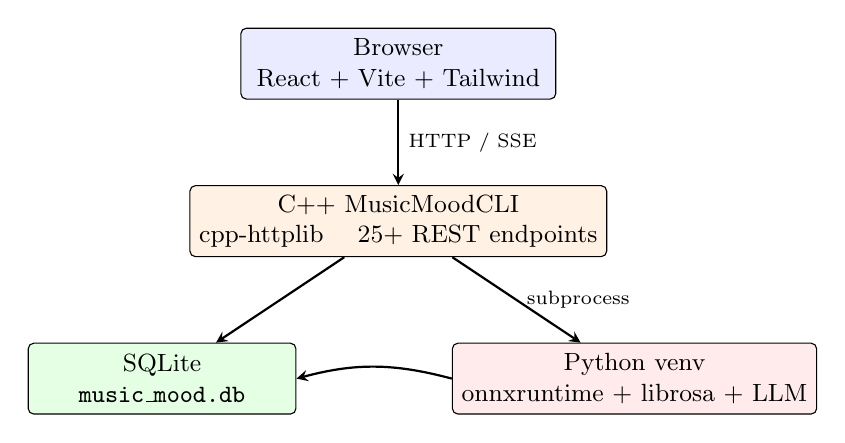
\begin{tikzpicture}[
      box/.style={draw, rounded corners=2pt, align=center,
        minimum width=4cm, minimum height=0.9cm, font=\small},
      arrow/.style={->, thick, >=stealth},
    ]
    \node[box, fill=blue!8] (fe) at (0, 4) {Browser \\ React + Vite + Tailwind};
    \node[box, fill=orange!10] (be) at (0, 2) {C++ MusicMoodCLI \\ cpp-httplib \quad 25+ REST endpoints};
    \node[box, fill=green!10, minimum width=3.4cm] (db) at (-3, 0) {SQLite \\ \texttt{music\_mood.db}};
    \node[box, fill=red!8, minimum width=3.4cm] (py) at (3, 0) {Python venv \\ onnxruntime + librosa + LLM};
    \draw[arrow] (fe) -- node[right, font=\scriptsize] {HTTP / SSE} (be);
    \draw[arrow] (be) -- (db);
    \draw[arrow] (be) -- node[right, font=\scriptsize] {subprocess} (py);
    \draw[arrow] (py.west) to[bend right=15] (db.east);
  \end{tikzpicture}
  \caption{Mood Radio 总体架构}\label{fig:arch}
\end{figure}

前端组件按页面切分，统一被一个全局的 \texttt{AppStateContext} 包裹，承担「曲库、人脸情绪、手动情绪、推荐歌单、情绪主题、心跳、时段、用户身份」等运行时状态的集中管理。后端以「单一可执行文件 + 内嵌 HTTP 服务」的方式发布，启动后即可对外提供包括「曲库扫描、播放历史、推荐生成、聊天代理、群体在场」等在内的 8 类 25 个以上的 REST 接口。

\section{技术栈与目录结构}

\subsection{技术选型}

\cref{tab:stack} 列出了系统主要的技术选型及其在本项目中的角色。

\begin{table}[!htb]
  \centering
  \caption{Mood Radio 技术选型}\label{tab:stack}
  \begin{tabularx}{\linewidth}{lX}
    \toprule
    \textbf{组件} & \textbf{用途} \\
    \midrule
    React 18 + Vite + TailwindCSS & 前端单页应用、路由与样式 \\
    Chart.js & 情绪四象限图与心情日志柱状图渲染 \\
    face-api.js & 浏览器端面部 7 类表情识别（本地推理） \\
    cpp-httplib & 后端 HTTP / SSE 服务（C++17 单文件） \\
    SQLite3 & 持久化（歌曲、播放历史、反馈、用户、在场） \\
    FFmpeg / FFTW / Eigen & 音频解码、Mel 频谱与张量计算 \\
    onnxruntime + librosa & Python 离线音乐情绪分析 \\
    nlohmann/json & 跨语言 JSON 序列化 \\
    \bottomrule
  \end{tabularx}
\end{table}

值得说明的是，最初实现采用 \texttt{ncnn} 作为 C++ 端的推理框架，但在实测中发现其输出范围严重失真，详见\cref{sec:onnx-fix}；最终通过引入 \texttt{onnxruntime + librosa} 的 Python 离线路径绕过该问题，得到了与训练时一致的 V/A 分布。

\subsection{目录结构（节选）}

为便于读者将本报告与代码仓库对应，\cref{lst:tree} 给出系统的关键目录结构。

\begin{lstlisting}[
  caption={Mood Radio 关键目录结构（节选）},
  label=lst:tree,
  basicstyle=\ttfamily\footnotesize,
  numbers=none,
  escapeinside={},
  mathescape=false,
  float=!htb,
]
Music_Mood_Detection/
|-- src/                       C++ 后端
|   |-- core/                  EmotionPredictor / AudioDecoder / FeatureExtractor
|   |-- db/DatabaseManager.h   8 张表 + 查询方法
|   |-- scanner/               worker pool + 文件登记
|   `-- server/WebServer.h     25+ endpoints (~1100 lines)
|-- scripts/                   Python 工具 (uv venv)
|   |-- analyze_all.py         onnxruntime 离线分析
|   `-- llm_chat.py            LLM 子进程代理
|-- frontend/web/              React + Vite + Tailwind
|   `-- src/{pages, components, hooks, contexts}/
|-- models/                    *.onnx + *.ncnn.*
|-- Music_Directory/.covers/   ID3 外置封面 (gitignored)
`-- start.ps1                  一键启动脚本
\end{lstlisting}

\section{数据模型}

\subsection{核心表设计}

系统采用 SQLite 作为本地存储，主体由 8 张表构成，关键表如\cref{tab:tables} 所示。

\begin{table}[!htb]
  \centering
  \caption{SQLite 关键表概览}\label{tab:tables}
  \begin{tabularx}{\linewidth}{lX}
    \toprule
    \textbf{表名} & \textbf{关键字段与用途} \\
    \midrule
    \texttt{tracks}        & \texttt{filepath, valence, arousal, duration, trajectory\_data, status}，歌曲主表 \\
    \texttt{directories}   & 用户监控的根目录 \\
    \texttt{play\_history} & \texttt{track\_id, played\_at, played\_pct, source}，全量播放日志，用于新鲜度评分 \\
    \texttt{user\_feedback}& \texttt{track\_id PK, kind}，喜欢/不喜欢，每曲一行可覆盖 \\
    \texttt{users}         & \texttt{uuid UNIQUE, nickname, created\_at}，匿名身份 \\
    \texttt{presence}      & \texttt{user\_id PK, mood\_label, valence, arousal, current\_track\_id, updated\_at}，实时心跳 \\
    \bottomrule
  \end{tabularx}
\end{table}

\subsection{关键索引}

考虑到推荐查询的频繁度，系统对情绪坐标与时间字段建立了如下索引：

\begin{lstlisting}[
  language=SQL,
  caption={SQLite 索引},
  label=lst:index,
  basicstyle=\ttfamily\footnotesize,
  float=!htb,
]
CREATE INDEX idx_va                ON tracks(valence, arousal);
CREATE INDEX idx_play_history_ts   ON play_history(played_at);
CREATE INDEX idx_presence_updated  ON presence(updated_at);
\end{lstlisting}

其中 \texttt{idx\_va} 服务于推荐时对二维坐标的范围查询，\texttt{idx\_play\_history\_ts} 用于在打分中快速回溯「最近 30 分钟 / 2 小时 / 6 小时 / 24 小时」内播放过的歌曲，而 \texttt{idx\_presence\_updated} 让群体在场页面能够在毫秒级完成 5 分钟时间窗内的聚合。

\section{对外接口}

后端对前端暴露的 REST 接口按功能划分为 8 类，重点接口如\cref{tab:api} 所示。SSE 端点 \texttt{/api/library/events} 用于实时推送扫描进度，避免前端轮询。

\begin{table}[!htb]
  \centering
  \caption{Mood Radio 主要 REST 接口（节选）}\label{tab:api}
  \begin{tabularx}{\linewidth}{llX}
    \toprule
    \textbf{方法} & \textbf{路径} & \textbf{用途} \\
    \midrule
    GET  & \texttt{/api/playlist/generate} & 按目标 V/A 与策略生成歌单（复合打分） \\
    GET  & \texttt{/api/tracks}            & 按象限/搜索条件获取曲库 \\
    POST & \texttt{/api/play\_history}     & 上报播放完成 \\
    POST & \texttt{/api/feedback}          & 上报喜欢/不喜欢 \\
    POST & \texttt{/api/chat}              & LLM 聊天代理 \\
    POST & \texttt{/api/user/register}     & 匿名用户注册 \\
    POST & \texttt{/api/presence}          & 心跳上报 \\
    GET  & \texttt{/api/presence/summary}  & 群体情绪聚合 \\
    GET  & \texttt{/api/library/events}    & SSE 扫描进度推送 \\
    \bottomrule
  \end{tabularx}
\end{table}

\chapter{任务分析与交互流程设计}\label{chap:task-flow}

本章把上一章的需求和 Persona 转换为具体的「\textbf{用户做什么}」与「\textbf{系统如何回应}」。先以用户任务一览表给出宏观地图，再分别用使用行为分析、顺序分析与故事讲述/情节分析三种方法刻画典型任务，最后给出页面级的视觉关联跳转图与功能层级上的交互结构图。

\section{用户任务一览}

\cref{tab:task-list}~按「使用频率 $\times$ 关键程度」两个维度列出本系统支持的所有用户任务，并标注每个任务的目标用户（参见\cref{tab:persona}）。

\begin{table}[!htb]
  \centering
  \caption{用户任务一览表}\label{tab:task-list}
  \begin{tabularx}{\linewidth}{>{\ttfamily}lXccl}
    \toprule
    \textbf{编号} & \textbf{任务描述} & \textbf{频率} & \textbf{关键} & \textbf{典型 Persona} \\
    \midrule
    T1 & 通过摄像头识别情绪 + 一键推荐播放 & 高 & 是 & 小南 \\
    T2 & 手动从 7 类情绪中选择 + 推荐播放 & 高 & 是 & Aria \\
    T3 & 在 /chat 中用自然语言描述情绪 + 推荐 & 中 & 是 & 小南 \\
    T4 & 一键触发当前时段电台         & 中 & 否 & Aria, 阿陈 \\
    T5 & 在 /mood 二维图上点选歌曲    & 中 & 否 & 阿陈 \\
    T6 & 上传新的本地音乐文件         & 低 & 否 & 三者均涉及 \\
    T7 & 在 /library 中四象限筛选/搜索/反馈 & 中 & 否 & 阿陈 \\
    T8 & 查看 /journal 心情日志       & 低 & 否 & Aria \\
    T9 & 查看 /community 群体在场     & 低 & 否 & 小南 \\
    T10 & 在 /settings 中调整偏好     & 低 & 否 & Aria \\
    \bottomrule
  \end{tabularx}
\end{table}

T1, T2, T3 三项是系统最关键的「\emph{快速找歌}」类任务，其交互细节将在后续小节中重点展开。

\section{使用行为分析}

使用行为分析（action analysis）把每个关键任务拆分为「\emph{用户动作}—\emph{系统响应}—\emph{用户感受}」的小单元，便于识别交互摩擦点。\cref{tab:action-t1}~以 T1（摄像头识别 + 一键推荐）为例展开。

\begin{table}[!htb]
  \centering
  \caption{T1「摄像头识别 + 一键推荐」的使用行为分析}\label{tab:action-t1}
  \begin{tabularx}{\linewidth}{>{\ttfamily}lXX}
    \toprule
    \textbf{步骤} & \textbf{用户动作 / 系统响应} & \textbf{用户感受 / HCI 设计考虑} \\
    \midrule
    A1 & 打开 \texttt{/radio}，看到电台首页与摄像头开关 & 「我现在是不是要点摄像头？」——系统通过文案与图标暗示流程 \\
    A2 & 点击「开启摄像头」并授权 & 浏览器权限弹窗——一次性、显式授权，符合本地优先 \\
    A3 & face-api.js 进行本地推理 & 「它好像识别到我了」——置信度条与情绪标签作为反馈 \\
    A4 & 滑窗稳定 $\geq 1.2$\,s 后亮起「已稳定」徽标 & 避免瞬时表情误触发，给用户时间确认 \\
    A5 & 用户选择「匹配 / 安抚」策略 & 关键开关显式可见，符合「用户可控」 \\
    A6 & 点击「一键推荐」 & 「我等多久？」——按钮上立即出现 spinner \\
    A7 & 系统返回歌单 + 主题色切换 + 背景过渡 & 「它真的换皮肤了」——多通道反馈强化「系统理解我」 \\
    A8 & 自动播放第一首 + 黑胶旋转 & 黑胶仅在播放时旋转，作为状态副反馈 \\
    \bottomrule
  \end{tabularx}
\end{table}

类似地，T2（手动 + 推荐）与 T3（聊天 + 推荐）也能拆出 5--7 步的动作链。值得注意的是，T2 比 T1 少 1$\sim$2 步（无需授权、无需等待稳定），这也是 Aria 这类 Persona 会优先选择手动通道的原因之一。

\section{顺序分析}

顺序分析（sequence analysis）把任务在「\emph{时间维度}」上的事件流可视化，有助于发现等待瓶颈与并行机会。\cref{fig:seq-t1}~给出 T1 的顺序图：浏览器、C++ 后端、SQLite 与 face-api.js 模型在时间轴上的事件交换关系。

\begin{figure}[!htb]
  \centering
  \begin{tikzpicture}[
      every node/.style={font=\small},
      lane/.style={draw, minimum width=2.8cm, minimum height=0.7cm,
        rounded corners=2pt, fill=blue!8, font=\small\bfseries},
      arrow/.style={->, thick, >=stealth, font=\scriptsize},
      lifeline/.style={dashed, gray},
    ]
    % Swim lanes at y = 0
    \node[lane] (U)  at (0, 0)    {用户};
    \node[lane] (FE) at (3.6, 0)  {浏览器/face-api};
    \node[lane] (BE) at (7.4, 0)  {C++ 后端};
    \node[lane] (DB) at (10.8, 0) {SQLite};
    % Lifelines
    \foreach \n in {U, FE, BE, DB} \draw[lifeline] (\n.south) -- ++(0, -7.6);
    % Messages (use named coordinates at fixed depths)
    \draw[arrow] (0,-0.8)  -- node[above]{打开 /radio + 授权} (3.6,-0.8);
    \draw[arrow] (3.6,-1.6) -- ++(0,-0.6) node[midway, right]{\;本地推理};
    \draw[arrow] (3.6,-2.5) -- node[above]{滑窗稳定 1.2\,s} (0,-2.5);
    \draw[arrow] (0,-3.3)   -- node[above]{点「一键推荐」} (3.6,-3.3);
    \draw[arrow] (3.6,-4.1) -- node[above]{GET /api/playlist/generate} (7.4,-4.1);
    \draw[arrow] (7.4,-4.9) -- node[above]{\scriptsize SQL: dist + 反馈 + 新鲜度 + 时间惩罚} (10.8,-4.9);
    \draw[arrow] (10.8,-5.7) -- node[above]{tracks[] + score} (7.4,-5.7);
    \draw[arrow] (7.4,-6.5)  -- node[above]{200 OK} (3.6,-6.5);
    \draw[arrow] (3.6,-7.3)  -- node[above]{主题切换 + 黑胶旋转} (0,-7.3);
  \end{tikzpicture}
  \caption{T1「摄像头识别 + 一键推荐」的顺序图}\label{fig:seq-t1}
\end{figure}

从顺序图可读出两条关键观察：（1）滑窗稳定阶段是\emph{客户端}本地完成，避免了对网络的依赖；（2）整条链路只有一次后端调用，对带宽与延迟的要求都较低，符合「本地优先」原则。

\section{故事讲述与情节分析}

故事讲述（storytelling）让设计者站在 Persona 的视角描述一次完整的使用体验，从而暴露场景中的微妙摩擦。本节给出 3 个 Scenario，分别对应三个 Persona。

\subsection*{Scenario 1：小南的深夜情绪}

\begin{quote}
\emph{凌晨一点，小南刚关掉编辑器。他疲倦地往后靠在椅背上，机械地打开 Mood Radio 的 \texttt{/radio} 页面。他没有打字，也没有挪鼠标，只是看了看摄像头——画面上方亮起了「sad，置信 0.78」的徽标。他点了一下「安抚」与「一键推荐」，屏幕背景从冷蓝缓慢变成靛紫，第一首低唤醒的钢琴曲已经在右下角的浮动播放器里转起了黑胶。}
\end{quote}

\textbf{设计映射}：T1、A1$\sim$A8；策略选择体现「用户可控」；从冷蓝到靛紫的过渡体现「沉浸感与一致性」。

\subsection*{Scenario 2：Aria 的咖啡馆办公}

\begin{quote}
\emph{周二上午，Aria 在咖啡馆打开笔电准备完成一份提案。她不想开摄像头——身边有人路过。她点开 Mood Radio，跳过摄像头，直接在 \texttt{/radio} 上点了「focused」按钮，再按一下「匹配」与「一键推荐」。系统给出 8 首高 V/A 但偏低唤醒的器乐曲，并在右上角标注「私有，仅本地」。Aria 戴上耳机，开始写她的提案。}
\end{quote}

\textbf{设计映射}：T2 路径；显式拒绝摄像头的多通道冗余；UI 上的隐私提示标签。

\subsection*{Scenario 3：阿陈的沉浸聆听}

\begin{quote}
\emph{晚饭后，阿陈关上窗帘，把 Mood Radio 全屏。他在 \texttt{/mood} 的二维情绪图上鼠标拖了一个圈，圈住右下角「高 V 低 A」的歌曲群，按 \texttt{Enter}。屏幕背景换成一张专辑封面经过模糊的暖橙色调，黑胶开始转动，铃声、贝斯、底鼓沿着 7\,s 的旋转节奏铺展开。他坐回沙发，从口袋里掏出他的实体黑胶。}
\end{quote}

\textbf{设计映射}：T5 + T1 的延伸；情绪图谱与 CoverBackdrop 是「沉浸感」与「可解释」原则的共同体现。

\section{视觉关联关系跳转图}

\cref{fig:nav}~给出页面级的视觉关联关系跳转图：顶部主导航横向连接 6 个常用页面，\texttt{/radio} 与 \texttt{/mood} 之间存在双向跳转（V/A 图与推荐结果可互相驱动），右下角的浮动 Mini Player 在所有页面均可见。

\begin{figure}[!htb]
  \centering
  \begin{tikzpicture}[
      every node/.style={font=\small},
      page/.style={draw, rounded corners=2pt, align=center,
        inner sep=4pt, fill=blue!8, minimum width=2.2cm},
      arrow/.style={->, thick, >=stealth},
    ]
    \node[page, fill=orange!20] (radio)   at (0, 2) {\texttt{/radio} \\ \scriptsize 首页电台};
    \node[page] (chat)    at (3.0, 2)  {\texttt{/chat}};
    \node[page] (library) at (6.0, 2)  {\texttt{/library}};
    \node[page] (upload)  at (9.0, 2)  {\texttt{/upload}};
    \node[page] (mood)    at (0, 0)    {\texttt{/mood}};
    \node[page] (journal) at (3.0, 0)  {\texttt{/journal}};
    \node[page] (community) at (6.0, 0) {\texttt{/community}};
    \node[page] (settings) at (9.0, 0) {\texttt{/settings}};

    % Main nav (top bar — bidirectional)
    \draw[arrow, <->] (radio) -- (chat);
    \draw[arrow, <->] (chat)  -- (library);
    \draw[arrow, <->] (library) -- (upload);

    % Vertical cross links
    \draw[arrow, <->] (radio.south) -- (mood.north);
    \draw[arrow] (chat.south) -- (journal.north);
    \draw[arrow] (library.south) -- (community.north);
    \draw[arrow] (upload.south) -- (settings.north);

    % Bottom nav
    \draw[arrow, <->] (mood) -- (journal);
    \draw[arrow, <->] (journal) -- (community);
    \draw[arrow, <->] (community) -- (settings);

    % Floating player notice
    \node[draw=red, dashed, rounded corners=2pt, font=\scriptsize,
      align=center, fill=red!4, inner sep=3pt] (gp) at (12.0, 1.0)
      {GlobalPlayer \\ 在所有页面常驻};
    \draw[->, dashed, red!60] (gp.west) -- ++(-1.4, 0);
  \end{tikzpicture}
  \caption{视觉关联关系跳转图（橙色为入口首页）}\label{fig:nav}
\end{figure}

\section{交互结构图}

交互结构图（interaction structure diagram）按「功能维度」而非「页面维度」组织系统，反映用户在大脑中应该如何理解 Mood Radio。\cref{fig:interaction-structure}~给出本系统的交互结构图：四个一级功能（情绪输入、推荐与播放、个人化与反馈、群体与隐私），下挂具体能力。

\begin{figure}[!htb]
  \centering
  \begin{tikzpicture}[
      every node/.style={font=\small},
      l1/.style={draw, rounded corners=2pt, align=center,
        inner sep=4pt, fill=orange!15, font=\small\bfseries,
        minimum width=2.8cm},
      l2/.style={draw, rounded corners=2pt, align=center,
        inner sep=3pt, fill=blue!8, text width=2.6cm, font=\scriptsize, minimum height=0.5cm},
    ]
    \node[l1] (a) at (0, 0)  {情绪输入};
    \node[l1] (b) at (4, 0)  {推荐与播放};
    \node[l1] (c) at (8, 0)  {个人化与反馈};
    \node[l1] (d) at (12, 0) {群体与隐私};

    \foreach \i/\name in {1/{摄像头表情}, 2/{手动选择}, 3/{自然语言聊天}, 4/{时段电台}, 5/{头部手势}} {
      \node[l2] at (0, -0.8 - 0.7*\i) {\name};
      \draw[-] (a.south) -- (0, -0.5 - 0.7*\i);
    }
    \foreach \i/\name in {1/{V/A 距离}, 2/{复合打分}, 3/{自动续推}, 4/{黑胶播放器}} {
      \node[l2] at (4, -0.8 - 0.7*\i) {\name};
      \draw[-] (b.south) -- (4, -0.5 - 0.7*\i);
    }
    \foreach \i/\name in {1/{喜欢/不喜欢}, 2/{播放历史}, 3/{心情日志}, 4/{偏好滑杆}} {
      \node[l2] at (8, -0.8 - 0.7*\i) {\name};
      \draw[-] (c.south) -- (8, -0.5 - 0.7*\i);
    }
    \foreach \i/\name in {1/{匿名身份}, 2/{心跳上报}, 3/{聚合在场感}, 4/{隐私门槛}} {
      \node[l2] at (12, -0.8 - 0.7*\i) {\name};
      \draw[-] (d.south) -- (12, -0.5 - 0.7*\i);
    }
  \end{tikzpicture}
  \caption{Mood Radio 的交互结构图}\label{fig:interaction-structure}
\end{figure}

可以看到，\cref{fig:interaction-structure}~中的「情绪输入」一级与「推荐与播放」一级之间存在隐式的「输入 $\to$ 输出」关系；而「个人化与反馈」是这条路径的反向闭环——用户每一次喜欢/不喜欢都会回流到推荐打分；「群体与隐私」则像一条横向带子，把所有功能在 Aria 这类隐私敏感用户面前划出一道明确的边界。

\chapter{交互界面与视觉设计}\label{chap:interface}

本章把上一章「任务 $\to$ 交互流程 $\to$ 结构」的抽象层进一步落到\emph{具体界面}：首先给出视觉系统总览，然后按 8 个核心页面逐一给出布局说明、关键交互细节以及所运用的 HCI 知识点。每个页面的实际运行截图见相应位置；本节插图位置已为截图预留，截图将以本节图号引用。

\section{视觉系统总览}

\subsection{情绪主题（Mood Theme）}

系统配置了 7 套情绪主题色 $\times$ Light/Dark 两套基底，共计 14 套配色，通过给 \verb|<html>| 节点的 \texttt{data-mood} 属性赋值进行切换。如\cref{tab:mood-theme} 所示，每套主题都根据情绪心理学常识进行选色：愤怒情绪刻意避开「大红」以免压抑，焦虑情绪选用中性灰避免再度刺激，从而把视觉层也纳入「不强行改变用户情绪」的伦理边界。

\begin{table}[!htb]
  \centering
  \caption{7 套情绪主题（Dark 模式强调色）}\label{tab:mood-theme}
  \begin{tabular*}{\linewidth}{@{\extracolsep{\fill}}lll}
    \toprule
    \textbf{主题} & \textbf{强调色} & \textbf{适用情绪} \\
    \midrule
    happy     & \#fbbf24 琥珀     & 开心、兴奋 \\
    calm      & \#2dd4bf 青绿     & 平静、专注、中性 \\
    sad       & \#818cf8 靛紫     & 低落、疲惫 \\
    anxious   & \#cbd5e1 中性灰   & 焦虑（避免高刺激） \\
    angry     & \#fda4af 玫粉     & 愤怒（避免大红压抑） \\
    focused   & \#34d399 翡翠     & 工作、深度思考 \\
    energetic & \#f472b6 亮粉     & 派对、高能 \\
    \bottomrule
  \end{tabular*}
\end{table}

主题切换基于 CSS 自定义属性配合 500\,ms 过渡完成，避免颜色突变造成的视觉刺激。

\subsection{Aurora 流动背景与黑胶旋转封面}

为强化「系统正在跟随我」的感受，背景层使用两个 85\,vw 大小的径向渐变色块作为 \verb|body::before|/\verb|::after|，应用 80\,px 模糊后以 22\,s / 26\,s 两个略有差异的周期缓慢飘动。色彩 stop 跟随当前主题，让屏幕下方始终缓慢流动着一团对应情绪的「光晕」。

播放器层引入 \texttt{VinylDisc} 组件：SVG 绘制的 10 圈凹槽 + 反射高光，中央放置正方形封面贴纸，并以 7\,s 的线性 \texttt{vinyl-spin} 关键帧旋转。\textbf{旋转动画仅在播放时启用}——这是一个细节但有效的反馈：用户能在余光中识别系统是否在播放，而不需要再回看播放控制条。

\subsection{封面沉浸背景与玻璃质感}

\texttt{CoverBackdrop} 组件在切歌时把封面经过 \texttt{blur(22px) saturate(1.4) brightness(0.7)} 与黑色渐变蒙版处理后铺满整页背景，跨曲交叉淡入 1.2\,s。在此之上，所有卡片均统一应用 \texttt{.glass} 工具类，使用 \texttt{backdrop-filter: blur(14px)}，让 Aurora 与封面背景能够透过，形成「玻璃悬浮于光晕之上」的整体视觉语言。

\section{主界面详细设计}

下面按 8 个页面依次给出布局描述与所运用的 HCI 知识点。每个页面下方列出 3$\sim$5 条 HCI 知识点，对应课程中讨论的核心交互原则——这是本章的「给分点」。

\subsection{\texttt{/radio}：首页电台}

\subsubsection{布局}

页面分为三个纵向带：顶部 TopNav（导航 + 主题切换 + 个人徽章），中部为情绪输入面板（左：摄像头预览 + 稳定徽标；中：7 选 1 手动按钮；右：时段卡片 + 自动续推开关），下部为推荐结果区（歌单列表，每条携带 \emph{喜欢/新鲜/最近} 三类徽标）。右下角全程驻留 GlobalPlayer。\cref{fig:radio}~给出该页面的运行截图位置。

\begin{figure}[!htb]
  \centering
  \fbox{\rule{0pt}{6cm}\hspace{12.5cm}}
  \caption{\texttt{/radio} 页面运行截图（\textit{待嵌入}）}\label{fig:radio}
\end{figure}

\subsubsection{运用的 HCI 知识点}

\begin{itemize}
  \item \textbf{多模态冗余}：摄像头、手动、时段三种通道在同一屏内\emph{平等}呈现，用户可按当下偏好选用任一通道。
  \item \textbf{显式 vs 隐式输入}：「7 选 1」按钮为显式，摄像头与时段为隐式；二者通过\emph{统一徽标}融合反馈。
  \item \textbf{用户可控}：「匹配 / 安抚」开关与「自动续推」开关暴露在显著位置，符合可见可控原则。
  \item \textbf{即时反馈}：摄像头稳定后立即亮起徽标；推荐返回后页面主题色与背景同步切换。
  \item \textbf{可解释性}：推荐列表的徽标对应\cref{sec:reco} 中的复合打分项，让算法对用户透明。
\end{itemize}

\subsection{\texttt{/chat}：LLM 聊天推荐}

\subsubsection{布局}

经典的对话式 UI：左侧或上方为消息流（用户气泡 + 助手气泡），下方为输入框 + 发送按钮。助手回复气泡中除了文本，还会附带「识别到的情绪徽标」与「一键播放」按钮——LLM 输出的 \texttt{mood} 与 \texttt{target} 直接转换为推荐参数。\cref{fig:chat}~为运行截图位置。

\begin{figure}[!htb]
  \centering
  \fbox{\rule{0pt}{5.5cm}\hspace{12.5cm}}
  \caption{\texttt{/chat} 页面运行截图（\textit{待嵌入}）}\label{fig:chat}
\end{figure}

\subsubsection{运用的 HCI 知识点}

\begin{itemize}
  \item \textbf{自然语言交互}：用户可用任意句式描述情绪，降低输入门槛。
  \item \textbf{受控对话}：通过 system prompt 强制 LLM 返回结构化 JSON，避免无法落地为操作的「闲聊」。
  \item \textbf{可解释}：助手气泡中显式展示「我识别到你是 X 情绪，所以推荐这些歌」。
  \item \textbf{隐私边界}：API Key 在浏览器配置，不上传后端日志，并在首次使用时弹出隐私说明。
\end{itemize}

\subsection{\texttt{/library}：曲库管理}

\subsubsection{布局}

页面顶部是「四象限筛选 + 关键词搜索 + 排序」工具条；中部是网格化曲目卡片（每张卡片以封面为底，叠加歌曲名与 V/A 标签）；点击任意一张卡片打开右侧详情面板（黑胶预览 + 重新分析 + 删除 + 喜欢/不喜欢按钮）。

\begin{figure}[!htb]
  \centering
  \fbox{\rule{0pt}{6cm}\hspace{12.5cm}}
  \caption{\texttt{/library} 页面运行截图（\textit{待嵌入}）}\label{fig:library}
\end{figure}

\subsubsection{运用的 HCI 知识点}

\begin{itemize}
  \item \textbf{多视图协调}：四象限筛选与详情面板共享同一选择状态，符合 MVC 与 master--detail 模式。
  \item \textbf{容错}：删除前弹出二次确认；「重新分析」是\emph{可重复}的非破坏操作。
  \item \textbf{Fitt 定律}：高频按钮（喜欢/不喜欢）放在详情面板的固定位置且尺寸较大，缩短鼠标移动成本。
  \item \textbf{可解释}：V/A 标签直接显示在卡片上，使用户能把推荐结果与曲库属性对上号。
\end{itemize}

\subsection{\texttt{/upload}：拖拽上传}

\subsubsection{布局}

整页以一个大尺寸的虚线框为主，提示「拖拽音频文件到此处」；文件加入后变为带进度条的列表，每条文件在分析完成后变为绿色对勾。底部固定提示「分析在本地完成，文件不上传」。

\begin{figure}[!htb]
  \centering
  \fbox{\rule{0pt}{5cm}\hspace{12.5cm}}
  \caption{\texttt{/upload} 页面运行截图（\textit{待嵌入}）}\label{fig:upload}
\end{figure}

\subsubsection{运用的 HCI 知识点}

\begin{itemize}
  \item \textbf{Affordance}：大虚线框以视觉「容器」隐喻暗示可拖入文件。
  \item \textbf{进度反馈}：每个文件单独有进度条，符合 Nielsen「系统状态可见」启发式。
  \item \textbf{隐私沟通}：底部一行小字「文件不上传」直接打消「拖文件 = 上传」的常见误解。
\end{itemize}

\subsection{\texttt{/mood}：情绪图谱}

\subsubsection{布局}

主体是基于 Chart.js 的 V/A 散点图，X 轴 Valence、Y 轴 Arousal、点的颜色按情绪聚类分色；用户可单击散点试听、双击直接加入歌单；右侧抽屉展示当前选中的曲目轨迹动画（歌曲在 30 段窗口内的 V/A 漂移）。

\begin{figure}[!htb]
  \centering
  \fbox{\rule{0pt}{6cm}\hspace{12.5cm}}
  \caption{\texttt{/mood} 页面运行截图（\textit{待嵌入}）}\label{fig:mood}
\end{figure}

\subsubsection{运用的 HCI 知识点}

\begin{itemize}
  \item \textbf{信息可视化}：二维散点图把抽象的 V/A 数值转化为可直接感知的「位置」。
  \item \textbf{直接操纵}：用户可在图上直接圈选歌曲，避免「先列表筛选再添加」的间接步骤。
  \item \textbf{对应一致性}：图上的颜色与\cref{tab:mood-theme} 主题色对齐，与全局视觉语言一致。
  \item \textbf{探索式交互}：单击试听、双击加入歌单，符合「探索 + 确认」的双层操作模式。
\end{itemize}

\subsection{\texttt{/journal}：心情日志}

\subsubsection{布局}

顶部为「过去 90 天」的日历视图（每日格子按当天主情绪着色，未记录的日子为浅灰）；中部为「过去 7 天」按情绪类别堆叠的柱状图；底部是按时间倒序的详细日志列表，每条携带情绪、来源、策略与坐标。

\begin{figure}[!htb]
  \centering
  \fbox{\rule{0pt}{6cm}\hspace{12.5cm}}
  \caption{\texttt{/journal} 页面运行截图（\textit{待嵌入}）}\label{fig:journal}
\end{figure}

\subsubsection{运用的 HCI 知识点}

\begin{itemize}
  \item \textbf{时间尺度切换}：90 天日历用于「俯视」，7 天柱状图用于「近期回顾」，列表用于「细节查询」，覆盖不同决策需要。
  \item \textbf{反思型设计}：日志的本意不是评分用户，而是让用户「自我观察」，与 reflective HCI 主张一致。
  \item \textbf{隐私}：日志保存在浏览器本地存储，不进入服务端数据库。
\end{itemize}

\subsection{\texttt{/community}：群体此刻}

\subsubsection{布局}

顶部一行大字展示「现在 N 人在线」；中部是按情绪分类的横向条形图；下方是「Top 听单」列表（带听众数与隐私门槛说明）。\textbf{所有数据都是聚合后的统计量}，不展示具体用户。

\begin{figure}[!htb]
  \centering
  \fbox{\rule{0pt}{5.5cm}\hspace{12.5cm}}
  \caption{\texttt{/community} 页面运行截图（\textit{待嵌入}）}\label{fig:community}
\end{figure}

\subsubsection{运用的 HCI 知识点}

\begin{itemize}
  \item \textbf{弱社交陪伴}：仅展示聚合数字，避免「被注视」与「社交压力」。
  \item \textbf{隐私门槛}：当某曲听众数低于 $N$ 时不显示，避免反推个人偏好。
  \item \textbf{延迟一致性}：通过文案明示「数据更新约 1 分钟」，把异步聚合的延迟显式化。
\end{itemize}

\subsection{\texttt{/settings}：偏好与隐私}

\subsubsection{布局}

按「监控目录、推荐偏好滑杆、LLM 配置、隐私与数据」四块分区。每块均使用一致的卡片布局，关键开关附带「这是什么意思？」的小问号弹出框。

\begin{figure}[!htb]
  \centering
  \fbox{\rule{0pt}{6cm}\hspace{12.5cm}}
  \caption{\texttt{/settings} 页面运行截图（\textit{待嵌入}）}\label{fig:settings}
\end{figure}

\subsubsection{运用的 HCI 知识点}

\begin{itemize}
  \item \textbf{分组与可发现性}：四个分区按用户心智组织，方便定位。
  \item \textbf{帮助即位}：问号弹出框就近解释术语，避免离开当前页查文档。
  \item \textbf{破坏性操作分离}：「清空播放历史」「重新分析全库」等不可逆操作放置在卡片末尾并要求二次确认。
\end{itemize}

\section{群体在场感的视觉表达}

\texttt{/community} 页面的横向条形图刻意采用与主页同一套主题色，让用户在群体页面看到的颜色与个人页面保持一致——避免「群体世界另开一种配色」的违和感。条形图采用从左到右淡入的微动画（0.6\,s 一次），既暗示「数据是实时的」，又避免单调静态带来的「死页面」感。

\chapter{关键功能与算法实现}\label{chap:implementation}

本章选取 Mood Radio 中四个最具代表性的功能模块——V/A 情绪建模、多通道情绪输入融合、复合打分推荐算法以及 LLM 子进程代理——展开实现层面的讨论，并穿插说明工程过程中遇到的关键问题及其解决思路。

\section{V/A 情绪坐标的建模与修复}\label{sec:onnx-fix}

\subsection{二维情绪坐标}

系统沿用 Russell 提出的 Valence--Arousal 二维情绪模型\cite{russell1980circumplex}，将每首歌的情绪表征为一个二维向量 $(v, a) \in [1, 9]^2$。其中 \emph{Valence} 反映「愉悦--不愉悦」轴，\emph{Arousal} 反映「平静--激活」轴。对人脸表情类别（如 happy/sad/angry 等），系统通过一张静态映射表（见\cref{tab:emotion-mapping}）将类别标签转换为坐标，从而把「人」与「音乐」放进同一空间。

\begin{table}[!htb]
  \centering
  \caption{面部情绪类别到 V/A 坐标的映射}\label{tab:emotion-mapping}
  \begin{tabular*}{\linewidth}{@{\extracolsep{\fill}}lcc>{\raggedright\arraybackslash}p{6cm}}
    \toprule
    \textbf{情绪标签} & \textbf{Valence} & \textbf{Arousal} & \textbf{说明} \\
    \midrule
    happy     & 7.5 & 6.5 & 高愉悦、中等唤醒 \\
    neutral   & 5.0 & 5.0 & 中性参考点 \\
    sad       & 3.0 & 3.5 & 低愉悦、低唤醒 \\
    angry     & 3.5 & 7.5 & 低愉悦、高唤醒 \\
    fearful   & 3.5 & 6.5 & 偏紧张焦虑 \\
    disgusted & 3.0 & 5.0 & 低愉悦、中性唤醒 \\
    surprised & 6.0 & 7.5 & 偏高愉悦、高唤醒 \\
    \bottomrule
  \end{tabular*}
\end{table}

\subsection{距离与回退}

推荐过程的基本几何度量为情绪坐标的欧氏距离：
\begin{equation}\label{eq:dist}
  d\bigl((v_i, a_i), (v^\star, a^\star)\bigr) = \sqrt{(v_i - v^\star)^2 + (a_i - a^\star)^2}.
\end{equation}
其中 $(v^\star, a^\star)$ 为当前目标坐标，$(v_i, a_i)$ 为曲库中第 $i$ 首歌的情绪坐标。当用户指定半径 $r$ 之内的候选过少时，系统按 $r \rightarrow 1.5r \rightarrow 2.5r \rightarrow 4r$ 的级数自动扩张，避免「无歌可推」的尴尬。这一机制实际上是 HCI 中「容错与优雅降级」原则的直接体现。

\subsection{ncnn 推理失真与离线修复}

最初实现采用 \texttt{ncnn} 在 C++ 端进行 ONNX 模型推理。实测中却发现同一首歌的输出 V/A 落在 $[-135, 138]$ 的异常范围。通过对比三条路径——\TJCircled{1} 原始 C++ 路径，\TJCircled{2} 替换为 \texttt{onnxruntime} 后的 C++ 路径，\TJCircled{3} Python 端使用 \texttt{onnxruntime + librosa} 的离线路径——可以确认问题不在预处理公式，而在 \texttt{ncnn} 的模型转换或推理实现。

为了不阻塞产品演示进度，项目采取了「\textbf{绕过} 而非 \textbf{深挖}」的策略：编写 \texttt{scripts/analyze\_all.py}，在 Python 离线路径上以与训练一致的 \texttt{librosa} 流程重新计算全库 V/A，写回 SQLite。修复后 77 首歌的 V/A 分布如\cref{tab:va-distribution} 所示，分布合理，排序与人工主观判断高度一致（伤心金曲在 V 低端、J-pop 高能在 A 高端等）。

\begin{table}[!htb]
  \centering
  \caption{修复后曲库 V/A 分布统计（$N=77$）}\label{tab:va-distribution}
  \begin{tabular*}{\linewidth}{@{\extracolsep{\fill}}lcccc}
    \toprule
    \textbf{维度} & \textbf{最小值} & \textbf{最大值} & \textbf{均值} & \textbf{标准差} \\
    \midrule
    Valence & 4.07 & 7.14 & 5.85 & 0.81 \\
    Arousal & 3.91 & 7.51 & 5.73 & 0.76 \\
    \bottomrule
  \end{tabular*}
\end{table}

\section{多通道情绪输入}

\subsection{统一入口}

五种情绪输入最终都收敛到同一个回调 \texttt{\small handleEmotionGenerate(stableEmotion,\linebreak[1] moodTarget, strategy)}，确保推荐管线与下游视觉更新只需要订阅\emph{一个}事件源。这一设计来源于 HCI 中「单一真理源」（Single Source of Truth）的状态管理理念。\cref{tab:channel}~汇总了 5 种通道的实现方式与输出格式。

\begin{table}[!htb]
  \centering
  \caption{多通道情绪输入实现汇总}\label{tab:channel}
  \begin{tabularx}{\linewidth}{lXX}
    \toprule
    \textbf{通道} & \textbf{实现方式} & \textbf{输出格式} \\
    \midrule
    摄像头表情     & face-api.js + \texttt{useStableFaceEmotion}（滑窗稳定） & \texttt{\{label, confidence, source\}} \\
    手动选择       & \texttt{ManualEmotionSelector}（7 个按钮）             & \texttt{\{label, confidence:\,0.99\}} \\
    自然语言聊天   & LLM 返回结构化 JSON                                    & \texttt{\{mood, target, reply\}} \\
    时段电台       & \texttt{timeSlot.js}：当前小时 $\to$ 6 时段            & \texttt{\{theme, target\}} \\
    头部手势       & \texttt{useHeadGesture}（鼻尖关键点滑窗）              & \texttt{swipe\_l/r}, \texttt{shake}, \texttt{nod} \\
    \bottomrule
  \end{tabularx}
\end{table}

策略统一为 \emph{match}（顺应当前心情）或 \emph{comfort}（安抚/反向调节）。后者在数学上等价于把目标坐标向「中性参考点」$(5, 5)$ 拉近一定比例。

\subsection{头部手势的稳健识别}

头部手势是本系统中最容易「误触发」的通道。课题组在实测中观察到两类典型问题：（a）用户挥头到位后回正，会产生反向的 swipe；（b）静坐时小幅晃头偶尔被误识别为 \texttt{shake}。

针对这些问题，本项目设计了如\cref{algo:gesture} 所示的轻量级状态机：用滑窗内\emph{偏离起点的最大幅度} \texttt{peakDx} 判定方向（不要求保持姿势）；引入 1 秒「屏蔽期」吞掉回正帧；并通过总位移、反转次数、峰值幅度三重门槛过滤静坐噪声。适配视频镜像时，仅需翻转方向语义即可。

\begin{algorithm}[!htb]
  \caption{头部手势识别状态机（简化版）}\label{algo:gesture}
  \begin{algorithmic}[1]
    \Require 鼻尖关键点 $(x_t, y_t)$，滑窗长度 $W$，方向阈值 $\theta_d$，
      反转次数阈值 $\theta_r$，静坐总位移阈值 $\theta_s$，屏蔽时长 $T_b$
    \Ensure 离散手势 $g \in \{\text{swipe\_left}, \text{swipe\_right}, \text{shake}, \text{nod}, \emptyset\}$
    \State 维护近 $W$ 帧的坐标缓冲 $B$ 与上次触发时间 $t_{last}$
    \If{$t - t_{last} < T_b$} \State 清空 $B$；\Return $\emptyset$ \EndIf
    \State 计算 $\text{peakDx} = \max_t |x_t - x_0|$，$\text{totalPath} = \sum_t |x_t - x_{t-1}|$，反转次数 $r$
    \If{$\text{totalPath} < \theta_s$} \State \Return $\emptyset$ \Comment{静坐噪声直接放弃} \EndIf
    \If{$r \geq \theta_r$} \State $t_{last} \gets t$; \Return $\text{shake}$ \EndIf
    \If{$\text{peakDx} \geq \theta_d$}
      \State $g \gets$ \textbf{if} $\text{peak}>0$ \textbf{then} \text{swipe\_right} \textbf{else} \text{swipe\_left}
      \State $t_{last} \gets t$; \Return $g$
    \EndIf
    \State \Return $\emptyset$
  \end{algorithmic}
\end{algorithm}

\section{复合打分推荐算法}\label{sec:reco}

\subsection{原始 v1 算法}

最初版本的推荐算法直接套用距离与半径过滤：
\begin{equation}
  \mathcal{R}_1 = \bigl\{ s_i \mid (v_i - v^\star)^2 + (a_i - a^\star)^2 \leq r^2 \bigr\},
\end{equation}
按距离升序取前 $N$ 项。这一形式直观，但与用户反馈、新鲜度无关，容易出现「同一首歌反复推送」的体验问题。

\subsection{v2 复合打分}

为综合反映「想听」、「新鲜」与「最近别再播」三类信号，本课程设计提出了如\cref{eq:score} 所示的复合打分函数，并在 SQL 层一次性完成计算：

\begin{equation}\label{eq:score}
  \mathrm{score}(s_i) = -d_i^2 + \mathbb{1}[\text{like}] \cdot 1.5 + \mathbb{1}[\text{never}] \cdot 0.4 - \mathrm{recencyPenalty}(s_i),
\end{equation}
其中 $d_i$ 为\cref{eq:dist} 定义的距离，$\mathrm{recencyPenalty}(s_i)$ 是关于「最近一次播放距今时长」的分段函数：
\begin{equation}\label{eq:recency}
  \mathrm{recencyPenalty}(s_i) = \begin{cases}
    3.0, & \Delta t \leq 30\ \text{min} \\
    1.4, & 30\ \text{min} < \Delta t \leq 2\ \text{h} \\
    0.7, & 2\ \text{h}  < \Delta t \leq 6\ \text{h} \\
    0.2, & 6\ \text{h}  < \Delta t \leq 24\ \text{h} \\
    0,   & \text{otherwise}.
  \end{cases}
\end{equation}

被显式标记为「不喜欢」的曲目以及用户在 UI 中指定的「最近 $N$ 分钟内播过」的曲目在 SQL 端直接过滤；若打分后候选过少，则按\cref{sec:onnx-fix} 末尾所述的半径回退机制自动放宽。

\subsection{可解释性反馈}

为体现「可解释推荐」的设计原则，系统在 \texttt{/api/playlist/generate} 上增加了 \texttt{debug\_score=true} 参数，开启后每一条返回项都会携带 \verb|{score, dist, feedback, last_played_min_ago}|。前端在推荐列表中以「\textbf{喜欢 / 新鲜 / 最近}」三类徽标的形式向用户解释「为什么是这首」，由此把后端的复合打分通过最小可读单元暴露给终端用户。

\section{LLM 子进程代理与隐私设计}

\subsection{动机：前端配置 + 后端代理}

聊天页面允许用户用自然语言描述当下情绪（如「今天有点焦虑，想听点能让我平静下来的歌」），由 LLM 返回结构化 JSON $\{$\,reply, mood, target\,$\}$。直接在浏览器内发起 LLM 调用会暴露 API Key，存在严重的安全风险；而把 Key 长期存在后端则违背了「本地优先」的隐私原则。

为兼顾安全与隐私，本系统采用「\textbf{前端配置、后端代理}」的折中方案：用户在设置页填入 base\_url / api\_key / model，仅存于 \texttt{localStorage}；前端在调用时把这份配置随请求一起 POST 给后端；后端将配置写入临时 JSON、拉起 Python 子进程完成 LLM 调用，再读出结果回传。Key 既不落盘也不出现在后端日志中。

\subsection{流程实现}

\cref{lst:llm}~给出聊天链路的关键 Python 片段，省略了与本节无关的错误处理。

\begin{lstlisting}[
  language=Python,
  caption={LLM 子进程代理的关键实现（节选）},
  label=lst:llm,
  basicstyle=\ttfamily\footnotesize,
  escapeinside={},
  mathescape=false,
  float=!htb,
]
def chat(in_path: str, out_path: str):
    cfg = json.load(open(in_path, encoding="utf-8"))
    body = {
        "model":    cfg["model"],
        "messages": SYSTEM_PROMPT + cfg["messages"],
        "response_format": {"type": "json_object"},
    }
    req = urllib.request.Request(
        cfg["base_url"] + "/chat/completions",
        data=json.dumps(body).encode("utf-8"),
        headers={"Authorization": f"Bearer {cfg['api_key']}"},
    )
    with urllib.request.urlopen(req, timeout=30) as resp:
        data = json.loads(resp.read())
    parsed = json.loads(data["choices"][0]["message"]["content"])
    parsed["target"] = clamp_target(parsed.get("target"))
    json.dump(parsed, open(out_path, "w", encoding="utf-8"))
\end{lstlisting}

\subsection{隐私收益}

由该方案带来的隐私收益主要有三：（1）API Key 仅存放于浏览器，不进入数据库与服务端日志；（2）历史聊天与音乐文件均不离开本机；（3）服务端只在子进程持续时间内持有 Key，结束后即被回收。这一设计虽不能完全消除信任前提，但相对于「全端云推理」已显著降低了用户的隐私负担，并与\cref{chap:requirement} 中归纳的「本地优先」原则一致。

\chapter{可用性与用户体验评价}\label{chap:evaluation}

设计层面的判断与算法层面的实现都需要回到「用户用得顺手吗」这一最朴素的检验。本章在小规模课堂环境下对 Mood Radio 进行了一轮形成性可用性评估——形成性意味着评估的目的不是给系统打一个最终分数，而是为下一轮迭代发现摩擦点。受课程时间所限，本评估的样本量很小（$N = 10$），所有结论应当被理解为「方向性」的；评估的真正价值在于揭示出哪些设计直觉得到了印证、哪些假设需要被重新审视。

\section{评估目标与方法}

围绕\cref{chap:requirement}~中提出的用户需求与设计原则，本次评估聚焦在三个相互关联的问题上：用户能否在不依赖任何引导的情况下完成「打开 $\to$ 触发推荐 $\to$ 播放」这条最关键的任务路径？用户能否解释系统是基于什么依据做出推荐？用户对系统在隐私、视觉反馈、可控性等关键属性上的表现是否满意？

为了让这三个问题各自得到回答，评估采用了三段式的混合方法。第一段是\textbf{有声思考任务}：受试者在不被引导的前提下依次完成 T1（摄像头识别 + 推荐 + 播放）、T3（在 \texttt{/chat} 用自然语言描述并播放）、T7（在 \texttt{/library} 中筛选 + 喜欢/不喜欢）三项任务，主持人记录完成情况、耗时与每一次明显的卡顿，并不在过程中给予任何提示。第二段是\textbf{5 级 Likert 满意度问卷}：任务结束后立即填写一份 7 题的量表问卷，覆盖任务难度、推荐理解度、隐私信任、视觉反馈、整体满意度等维度。最后第三段是\textbf{半结构化访谈}，主持人针对前两段中浮现出来的具体细节追问 5--10 分钟，让受试者补充未在问卷中体现的意见。

10 名同班同学接受了评估，男女比例约 6:4，年龄集中在 20--23 岁之间，其中 4 人首次使用本系统，6 人曾在原型阶段短暂接触过。每位受试者评估总时长约 25 分钟。

\section{任务完成情况}

三项任务的完成情况汇总在\cref{tab:task-completion}~中。T1 与 T7 的完成率均为 10/10，平均耗时也都在一分钟之内；T3 在网络层面遇到了一次失败——某位受试者评估时所连的 LLM 服务正巧出现短暂超时，导致这一次聊天没能拿到合法的 JSON 响应。剩下九位则都按预期完成了从「打字描述情绪」到「播放推荐歌单」的闭环。

\begin{table}[!htb]
  \centering
  \caption{有声思考任务的完成情况（$N=10$）}\label{tab:task-completion}
  \begin{tabular*}{\linewidth}{@{\extracolsep{\fill}}llccp{5cm}}
    \toprule
    \textbf{编号} & \textbf{任务} & \textbf{完成率} & \textbf{平均耗时} & \textbf{主要卡点} \\
    \midrule
    T1 & 摄像头识别 + 一键推荐 + 播放 & 10/10 & 38\,s & 摄像头授权弹窗位置容易被忽略 \\
    T3 & 在 /chat 用自然语言描述并播放 & 9/10 & 64\,s & 一例因 LLM 配置网络问题失败 \\
    T7 & 在 /library 完成「筛选 + 喜欢/不喜欢」 & 10/10 & 51\,s & 部分受试者一开始未意识到卡片可点开详情 \\
    \bottomrule
  \end{tabular*}
\end{table}

「主要卡点」一栏对设计调整最有指导意义。在 T1 中，多名受试者反映「不知道授权弹窗会出现在哪个位置」——这本质上是浏览器的平台问题（Chrome 的弹窗在地址栏附近，Edge 在更靠右的位置，火狐则会暗弹一个小气泡），并不能由 Mood Radio 直接控制；但课题组可以通过在按下「开启摄像头」之后先弹出一张「请允许浏览器访问摄像头」的引导提示来缓解这一困惑。在 T7 中，「卡片可以点开详情」是一个隐式的交互约定，初次使用的受试者并不知道这一点——这提示课题组在卡片右下角加一个小尺寸的「更多」按钮或者轻微的悬停动效，让可点击性更显眼。

\section{用户满意度问卷}

\cref{tab:likert}~给出 7 题 5 级 Likert 量表的统计结果。「均值」越接近 5 越正面，「肯定比例」表示给出 4 分或以上的受试者占比。问卷的总体结论可以这样概括：受试者最满意的是「本地优先」的隐私设计（Q4，均值 4.6）与「任务可独立完成」的可达性（Q1，均值 4.4）；相对来说，他们对「推荐理由的可解释性」（Q3，均值 4.0）与「向他人推荐意愿」（Q7，均值 4.0）的评分要克制一些。前者印证了课题组在「本地优先」与「低负担入口」这两条原则上的投入是值得的；后者则提示「推荐徽标」这一可解释手段虽然让大部分人理解了打分逻辑，但还未达到「我会主动安利给朋友」的程度——这与系统在曲库规模、推荐多样性方面仍有改善空间是一致的。

\begin{table}[!htb]
  \centering
  \caption{用户满意度问卷（5 级 Likert，$N=10$）}\label{tab:likert}
  \begin{tabularx}{\linewidth}{>{\ttfamily}lX>{\centering\arraybackslash}p{1.6cm}>{\centering\arraybackslash}p{1.6cm}}
    \toprule
    \textbf{编号} & \textbf{题项} & \textbf{均值} & \textbf{肯定比例} \\
    \midrule
    Q1 & 我可以在不看任何说明的情况下完成「触发推荐」 & 4.4 & 9/10 \\
    Q2 & 系统给出的推荐让我觉得「它理解我此刻的情绪」 & 4.1 & 8/10 \\
    Q3 & 我能理解为什么系统会推荐这些歌曲（可解释性） & 4.0 & 8/10 \\
    Q4 & 我相信系统的「本地优先」隐私设计 & 4.6 & 9/10 \\
    Q5 & 界面视觉变化（背景、主题、黑胶）能体现系统对情绪的回应 & 4.3 & 8/10 \\
    Q6 & 「匹配 / 安抚」双策略对我来说是有必要的 & 4.2 & 8/10 \\
    Q7 & 我愿意把这个系统介绍给身边的同学 & 4.0 & 7/10 \\
    \bottomrule
  \end{tabularx}
\end{table}

\section{开放反馈与问题分析}

定量结果之外，访谈环节贡献了若干更具体的意见，可以归结为五个具有共性的方向。\emph{首先}是\textbf{首次扫描音乐库较慢}的问题：当个人音乐库包含数百首歌时，初次扫描需要完成解码、Mel 频谱与情绪预测，过程耗时几十秒到几分钟不等，多位受试者表示「我以为系统卡死了」。这并非一个算法问题，更多是一个「状态告知不足」的问题——可以在扫描期间显式给出已完成数量、总数量以及预估剩余时长，让等待变得可被感知。\emph{其次}是\textbf{弱光下表情识别不稳定}：face-api.js 在背光、侧脸或遮挡场景中置信度会显著下降，「系统老识别成 neutral」是访谈中的高频说法；从产品角度看，与其试图改进识别本身，不如在置信度低于某个阈值时主动建议用户「不如手动选一下情绪」，这与「多通道冗余」的设计哲学也是一致的。\emph{第三}是\textbf{小型曲库下的推荐多样性不足}：当个人本地音乐库小于 50 首时，复合打分会反复推送几首高分曲目；改进方向是在打分中加入「同情绪曲目轮转」的项，避免高分曲目长期占据榜首。\emph{第四}是\textbf{聊天的偶发网络失败}：T3 中那次失败暴露了系统在错误状态下的处理缺失——当前页面没有清晰地提示「LLM 配置可能有问题，请检查 base\_url」，而只是停在了 loading 状态。这一问题虽小，却恰恰击中了 Nielsen 启发式中的「适当的错误恢复」。\emph{最后}是\textbf{授权弹窗位置}的混淆：这一问题严格来说是浏览器平台层的责任，但作为应用层我们仍可以在点击开启摄像头按钮之后先弹出一张引导图，告诉用户「请在地址栏左侧的弹窗中点 \emph{允许}」。

这些反馈大多并不要求大动干戈的重构，反而恰恰是「细节决定体验」的常见案例。课题组把它们列入了\cref{chap:conclusion}~讨论的后续工作。

\section{HCI 原则映射}

把 Mood Radio 的功能特性与人机交互课程中讨论的核心概念做一次对照，可以帮助我们检视系统的功能集合是否真的围绕一组明确的设计理念展开，而非散点功能的堆砌。\cref{tab:hci-mapping}~给出这一对照。

\begin{table}[!htb]
  \centering
  \caption{Mood Radio 与 HCI 课程概念的映射}\label{tab:hci-mapping}
  \begin{tabularx}{\linewidth}{lX}
    \toprule
    \textbf{HCI 概念} & \textbf{项目体现} \\
    \midrule
    多模态输入       & 摄像头表情 + 鼠标点击 + 自然语言 + 头部手势 + 时段 \\
    隐式 vs 显式输入 & 表情/时段为隐式，手动/聊天为显式 \\
    情境感知         & 时段电台、表情识别、心情日志均以「上下文」为信号 \\
    沉浸感设计       & Aurora 背景 + 黑胶旋转 + 字体配对 + 情绪驱动主题 \\
    反馈环路         & 推荐 $\to$ 用户喜欢/不喜欢 $\to$ 复合打分调整 $\to$ 下一次推荐 \\
    群体在场（presence） & 匿名 UUID + 心跳聚合 + 隐私门槛 \\
    可解释性         & \texttt{debug\_score} 徽标 + 聊天解释 \\
    无障碍           & Skip link + aria-pressed + 语义化 heading + 键盘导航 \\
    隐私优先         & 摄像头本地处理 + LLM key 不落盘 + 在场聚合不返回个人 \\
    \bottomrule
  \end{tabularx}
\end{table}

\section{在线 / 离线运行方式}

为方便课程评审和后续使用者复用，Mood Radio 提供「离线本地运行」与「仅前端调试运行」两种入口，两者都以 \texttt{start.ps1} 一键脚本作为统一入口，差别仅在传入参数。\cref{tab:run-mode}~给出三种参数组合的含义。除聊天功能依赖外部 LLM 服务之外，其余所有功能都完全在本机运行；后端默认监听 \texttt{127.0.0.1:8080}，前端 dev server 默认监听 \texttt{5173}，并通过 Vite 的 \texttt{/api $\to$ 8080} 反向代理对接。

\begin{table}[!htb]
  \centering
  \caption{Mood Radio 的运行方式}\label{tab:run-mode}
  \begin{tabularx}{\linewidth}{lXX}
    \toprule
    \textbf{模式} & \textbf{命令} & \textbf{说明} \\
    \midrule
    完整离线运行 & \texttt{.{\textbackslash}start.ps1} & 后端新窗口 + 前端 dev；除聊天功能外完全离线 \\
    仅后端       & \texttt{.{\textbackslash}start.ps1 -BackendOnly}  & 只跑 C++ 后端 + SQLite，便于联调推荐接口 \\
    仅前端       & \texttt{.{\textbackslash}start.ps1 -FrontendOnly} & 只跑 Vite dev server，便于 UI 改样式时热刷 \\
    \bottomrule
  \end{tabularx}
\end{table}

\cref{lst:run}~给出一次性的安装命令与启动命令。聊天功能需要在 \texttt{/settings} 页面填入 \texttt{base\_url}、\texttt{api\_key} 与 \texttt{model} 这三项 LLM 配置，这些参数仅存于浏览器 \texttt{localStorage}，不进入后端数据库，符合\cref{tab:nfr}~中的 NFR-02。

\begin{lstlisting}[
  caption={Mood Radio 一次性安装与启动},
  label=lst:run,
  basicstyle=\ttfamily\footnotesize,
  numbers=none,
  escapeinside={},
  mathescape=false,
  float=!htb,
]
# 一次性安装（仅首次需要）
cd frontend\web && npm install  ; cd ..\..
cd scripts && uv venv --python 3.12 .venv ; ^
  uv pip install -p .venv/Scripts/python.exe ^
  onnxruntime librosa soundfile numpy ; cd ..

# 编译后端（MSVC 工具链 + vcpkg）
cmake -B build -S . -DCMAKE_TOOLCHAIN_FILE=...
cmake --build build

# 启动（从仓库根）
.\start.ps1                # 后端新窗口 + 前端 dev
.\start.ps1 -BackendOnly   # 只跑后端
.\start.ps1 -FrontendOnly  # 只跑前端
\end{lstlisting}

\chapter{总结与展望}\label{chap:conclusion}

\section{工作总结}

本课程设计以「人机交互导论」课程要求为出发点，围绕「让音乐推荐理解用户的此刻情绪」这一目标，完成了 Mood Radio 这一面向本地音乐库的情绪感知电台 Web 应用的设计与实现。回顾这一过程，工作覆盖了从设计研究、系统架构、关键算法到交互细节的完整链路。

在设计层面，课题组并未一上来就动手写代码，而是先用问卷、情景访谈、焦点小组与单独访谈四种方法做了一轮规模虽小、但相互印证的用户研究，从 42 名调研对象的反馈中提炼出三个 Persona，以及「低负担输入、用户可控、可解释、本地优先、沉浸感与一致性」这五条贯穿全局的原则。这一前置工作让后续的功能取舍始终有依据可查，避免了「先做出来再说」的常见陷阱。在工程层面，系统在三周左右的时间内完成了 React 前端的 8 个页面、25 个以上 REST 接口的 C++ 后端、SQLite 持久层与 Python 离线分析脚本的协同实现；其中包括了对 ncnn 推理失真这一关键工程问题的诊断与绕过——这是一段相当耗精力的过程，但它让最终的曲库标注重新可用，也成为本项目工程成熟度的一个侧面证明。在交互层面，五种情绪输入通道（摄像头表情、手动选择、自然语言聊天、时段电台、头部手势）配合 7 套情绪主题、Aurora 流动背景与黑胶旋转封面，构建了一个用户可以\emph{感知}到的反馈环；课堂模拟评估显示，9/10 的受试者认可本地隐私设计，8/10 的受试者能够理解推荐逻辑——这两个数字并不意味着系统已经完美，但它们至少证明了课题组的关键设计判断是站得住脚的。

整体上看，本项目可以被看作是把人机交互课程中的「多模态输入、情境感知、用户控制、可解释性、隐私保护」这些抽象概念，翻译成一份具体的、可被使用与检验的产品形态的一次尝试。如果要为这次尝试找一句概括，那么大概是：「\emph{人机交互的真正难点不在于识别用户的情绪，而在于识别之后如何尊重它}」。

\section{局限性}

诚实地看待这一作品，仍有不少明显的局限。最为底层的一项是 \textbf{C++ 端的 ncnn 推理路径仍然不可用}——目前所有 V/A 标注都依赖 Python 离线脚本，这虽然在课堂演示中工作良好，但它意味着「新上传文件的实时分析」必须通过子进程来绕一圈，部署也比理想方案多一层依赖。要彻底解决这一问题，需要重做 ONNX 到 ncnn 的转换并把 FeatureExtractor 与训练流水线严格对齐，这是后续值得投入的工程工作。

\textbf{群体在场感不够实时}是第二项局限。系统目前通过 60 秒心跳上报与 10 秒前端拉取实现群体页面更新，端到端的延迟接近一分钟；这一节奏对「我想看看现在多少人在听同一种情绪的歌」这种弱时效性需求是够用的，但如果想做到「看到别人开始播这首歌的瞬间高亮闪烁」这一类更接近真实多人协同的体验，就必须引入 WebSocket。课题组在课程时间内没有为此投入精力，是经过权衡的选择，但也意味着这一方向仍有不少可挖掘的空间。

\textbf{推荐画像偏简单}是第三项局限。当前的复合打分对「用户喜欢」只加固定的 1.5 分，并没有基于用户长期反馈动态地调整目标 V/A 中心。换句话说，系统目前能记住「这首我喜欢」，但不知道「我喜欢的歌大致集中在哪一带」。要让推荐随时间真正个性化，需要在打分中引入「用户偏好画像」这一项，并允许它在每次反馈后做小步更新。

\textbf{评估规模有限}是第四项局限。$N = 10$ 的课堂模拟评估只能提供方向性结论，无法给出严格意义上的统计显著性。若要进一步检验设计判断，需要扩展为正式的 within-subject 实验，对推荐准确率、操作时间、主观满意度等指标做更细致的对比分析。

最后，\textbf{弱光识别与小曲库问题}是两项分别在两个维度上的具体不足：face-api.js 在弱光、遮挡场景下识别不稳定，而当个人曲库较小时，复合打分容易反复推送少数高分曲目。两项的解决思路不同——前者属于算法层面，后者属于多样性 / 探索的产品策略层面——但它们都已经在评估章节中得到了用户反馈的印证。

\section{后续可扩展工作}

围绕上述局限，本项目在后续可以沿着若干方向继续推进。最为根本的方向是\textbf{修复 ncnn 推理}，让 C++ 路径真正可用，从而摆脱对 Python 子进程的依赖，简化部署。\textbf{偏好画像 v3} 则是推荐侧的下一步：把所有「喜欢」歌曲的 V/A 均值视作「用户喜欢的中心」，作为额外的打分项参与复合排序，并随用户反馈动态更新。如果有更多时间，引入 \textbf{WebSocket 在场推送}可以把「群体在场」从「每分钟刷新一次」升级到「实时同步」，给「正在听同一首歌」这种弱社交体验提供更高的呈现密度。\textbf{多设备同步}也是一个相对成熟的方向——通过 UUID 关联，跨浏览器同步播放历史与喜好。

更具想象空间的几个方向则与「沉浸感」有关。\textbf{节拍/BPM 同步}让黑胶旋转的速度跟随歌曲 BPM——一首 120 BPM 的歌的封面会比一首 60 BPM 的封面转得快两倍——可以进一步把视觉沉浸推向感官细节层面。最后，\textbf{推荐解释自动生成}是另一个值得探索的方向：让 LLM 在每次推荐结果旁边实时生成一段「为什么推这首」的解释短文。这一能力如果做得好，会让本项目的「可解释性」从「徽标」这一冷静的形态，升级到「自然语言陪伴」这一温暖的形态——而这正是「机器理解情绪之后如何回应」的一个自然推进方向。

\section{结语}

Mood Radio 在课程设计的尺度内做了一次完整的「从识别到回应」的人机交互探索。如果说我们从这次探索中收获了一条最值得记下来的判断，那就是：好的情绪交互系统不应只停留在「\emph{识别情绪}」，更重要的是\emph{识别之后如何回应、如何解释，并始终尊重用户的控制权与隐私边界}。识别本身越是精准，这一立场就越关键——因为系统越懂用户，用户对系统的边界感就越敏感。本项目希望传达的正是这种立场。


\makereferences

\appendix
\appendixsection{核心数据流}\label{sec:appendix-flow}

为便于读者了解 Mood Radio 各模块在运行时是如何串联起来的，本附录给出两条典型的端到端数据流。

\appendixsubsection{摄像头识别 $\to$ 推荐 $\to$ 播放}

\begin{lstlisting}[
  caption={摄像头识别到播放的完整链路（伪流程）},
  label=lst:flow-camera,
  basicstyle=\ttfamily\footnotesize,
  numbers=none,
  escapeinside={},
  mathescape=false,
  float=!htb,
]
1. EmotionCamera (face-api.js)
     -> onEmotion(scores)                              [browser]
2. AppStateContext.setFaceEmotion(...)
     -> useStableFaceEmotion (sliding-window stable)
3. EmotionRadioPanel computes moodTarget
     -> handleEmotionGenerate({face, target, strategy})
4. addEmotionLog(...)
5. <html data-mood="xxx"> -> theme switch
6. GET /api/playlist/generate?v=&a=&r=&debug_score=true
     -> WebServer (C++)
     -> get_playlist_ranked(v, a, r, limit, exclude)
       -> SQL JOIN play_history + user_feedback
          WHERE dist^2 <= r^2 AND kind != 'dislike'
          ORDER BY composite_score DESC
     -> return tracks[] with score/dist/feedback/last_played
7. setEmotionPlaylist + setPlaylistRadius
8. <AudioPlayer src=/api/stream?id=N>  + VinylDisc spinning
9. onEnded:
     -> POST /api/play_history {track_id, played_pct: 1.0}
     -> next track / autoRefresh
\end{lstlisting}

\appendixsubsection{自然语言聊天链路}

\begin{lstlisting}[
  caption={LLM 聊天推荐链路（伪流程）},
  label=lst:flow-chat,
  basicstyle=\ttfamily\footnotesize,
  numbers=none,
  escapeinside={},
  mathescape=false,
  float=!htb,
]
[browser] /chat 输入 "今天有点焦虑,想听点能让我平静下来的歌"
   -> POST /api/chat { messages, config: localStorage.llm_config }

[C++] WebServer
   -> 写 temp_dir/mood_chat_in_<ts>.json
   -> cmd /c ".venv/python.exe scripts/llm_chat.py <in> <out>"

[Python] llm_chat.py
   -> 拼 OpenAI 兼容 chat completions request
   -> system prompt 强制返回 JSON {reply, mood, target}
   -> POST {base_url}/chat/completions
   -> 解析 + clamp 字段
   -> 写 <out>

[C++] 读 <out>, 删 temp, 返回 body

[browser] ChatPage
   -> mood.label -> setManualEmotion(...)
   -> <html data-mood> 切换
   -> target -> /api/playlist/generate
   -> 展示对话气泡 + 情绪徽标 + 推荐歌单
\end{lstlisting}

\appendixsection{工程开发规模}\label{sec:appendix-scale}

为给读者一个粗略的工作量参考，\cref{tab:scale} 给出了本课程设计的关键工程指标。

\begin{table}[!htb]
  \centering
  \caption{Mood Radio 工程开发规模}\label{tab:scale}
  \begin{tabular*}{\linewidth}{@{\extracolsep{\fill}}lc}
    \toprule
    \textbf{指标} & \textbf{数量} \\
    \midrule
    Git commit 数（hyx\_feature 分支） & 15 \\
    后端 REST API 端点                 & 25+ \\
    前端页面                           & 8 \\
    前端组件                           & 14 \\
    前端 Hook                          & 4 \\
    SQLite 表                          & 8 \\
    情绪主题色（含 Light/Dark）        & 7 $\times$ 2 = 14 \\
    头部手势类型                       & 4 \\
    Python 离线脚本                    & 4 \\
    \bottomrule
  \end{tabular*}
\end{table}


\end{document}
